\documentclass[article]{jss}

%% -- LaTeX packages and custom commands ---------------------------------------

%% recommended packages
\usepackage{thumbpdf,lmodern}

%% additional packages
\usepackage{amssymb,amsmath}

%% new custom commands
\newcommand{\class}[1]{`\code{#1}'}
\newcommand{\fct}[1]{\code{#1()}}

%% For Sweave-based articles about R packages:
%% need no \usepackage{Sweave}



%% -- Article metainformation (author, title, ...) -----------------------------

%% - \author{} with primary affiliation
%% - \Plainauthor{} without affiliations
%% - Separate authors by \And or \AND (in \author) or by comma (in \Plainauthor).
%% - \AND starts a new line, \And does not.
\author{Lennart Oelschl\"ager \\Bielefeld University \And Dietmar Bauer\\Bielefeld University}
\Plainauthor{Lennart Oelschl\"ager, Dietmar Bauer}

%% - \title{} in title case
%% - \Plaintitle{} without LaTeX markup (if any)
%% - \Shorttitle{} with LaTeX markup (if any), used as running title
\title{\pkg{RprobitB}: Bayes Estimation of Discrete Choice Behavior Heterogeneity via Probit Models in \proglang{R}}
\Plaintitle{RprobitB: Bayes Estimation of Discrete Choice Behavior Heterogeneity via Probit Models in R}
\Shorttitle{RprobitB}

%% - \Abstract{} almost as usual
\Abstract{
\pkg{RprobitB} is an \proglang{R} package for Bayes estimation of probit models with a special focus on modeling choice behavior heterogeneity. In comparison to competing packages it places a focus on approximating the mixing distribution via a latent mixture of Gaussian distributions and thereby providing a classification of deciders. It provides tools for data management, model estimation via Markov Chain Monte Carlo Simulation, diagnostics tools for the Gibbs sampling and a prediction function. This paper demonstrates the functionalities of \pkg{RprobitB} on known choice datasets and compares estimation results across packages.
}

%% - \Keywords{} with LaTeX markup, at least one required
%% - \Plainkeywords{} without LaTeX markup (if necessary)
%% - Should be comma-separated and in sentence case.
\Keywords{discrete choice, probit models, heterogeneity, Bayes estimation, \proglang{R}}
\Plainkeywords{discrete choice, probit models, heterogeneity, Bayes estimation, R}

%% - \Address{} of at least one author
%% - May contain multiple affiliations for each author
%%   (in extra lines, separated by \emph{and}\\).
%% - May contain multiple authors for the same affiliation
%%   (in the same first line, separated by comma).
\Address{
  Lennart Oelschl\"ager\\
  Department of Business Administration and Economics\\
  Bielefeld University\\
  Postfach 10 01 31\\
  E-mail: \email{lennart.oelschlaeger@uni-bielefeld.de}
}

\begin{document}
%% I have no idea what this does. Maybe we need this in the future.
%% \SweaveOpts{concordance=TRUE}

%% -- Introduction -------------------------------------------------------------

%% - In principle "as usual".
%% - But should typically have some discussion of both _software_ and _methods_.
%% - Use \proglang{}, \pkg{}, \fct{} and \code{} markup throughout the manuscript.
%% - If such markup is in (sub)section titles, a plain text version has to be
%%   added as well.
%% - All software mentioned should be properly \cite-d.
%% - All abbreviations should be introduced.
%% - Unless the expansions of abbreviations are proper names (like "Journal
%%   of Statistical Software" above) they should be in sentence case (like
%%   "generalized linear models" below).

\section{Introduction}
\label{sec:introduction}

%% Short introduction
The multinomial probit model is one of the most widely-used statistical models to explain the choices that individuals make among a discrete set of alternatives, which is of central interest in many scientific areas, for example in transportation and marketing. In many such choice scenarios it is reasonable to assume, that the preferences of the decision makers are non-homogeneous. Based on personal characteristics, deciders generally weight attributes like time and cost differently. Heterogeneity in choice behavior can be modeled using mixing distributions for the coefficients. Recently, Oelschlaeger and Bauer proposed a new instrument for approximating the underlying mixing distribution that combines Bayes estimation and semi-parametric methods. This paper presents the implementation of the methodology in the \proglang{R} package \pkg{RprobitB}.

%% Overview RUMs
Traditionally, discrete choice models are interpreted as random utility models, including the multinomial logit (MNL) and the multinomial probit (MNP) model as the most prominent members. The MNL model affords straightforward analysis but suffers from the well-known independence of irrelevant alternatives assumption. In contrast, the MNP model avoids this assumption, which however comes at the price of more complex parameter estimation, cf. \cite{Train:2009}. In their basic form, these models often fail to take into account heterogeneity of individual deciders, cf. \cite{Train:2009}, Chapter 6, or \cite{Train:2016}. A concrete example of heterogeneous preferences is constituted by the value of travel time, cf. \cite{Cirillo:2006}. Modeling heterogeneity in preferences is indispensable in such cases and has been elaborated in both the MNL and the MNP model by imposing mixing distributions on the coefficients, cf. \cite{Train:2009} and \cite{Bhat:2011}.

%How are the mixing distribution specified currently?
Specifying these mixing distributions is an important part of the model selection. In absence of alternatives, it has been common practice so far to try different types of standard parametric distributions (including the normal, log-normal, uniform and tent distribution) and to perform a likelihood value-based model selection, cf. \cite{Train:2009}, Chapter 6. Aiming to capture correlation patterns across parameters, \cite{Fountas:2018} and \cite{Fountas:2019} apply multivariate normal mixing distributions in their probit models, which however comes at the price of imposing the rather strong normality assumption on their parameters.

In order to alleviate these restrictions \cite{Train:2016} proposes a non-parametric approach based on grid methods. Building on the ideas of \cite{Train:2016} and \cite{Bhat:2018} recently \cite{Bauer:2019} introduced procedures for non-parametrically estimating latent class mixed multinomial probit models where the number of classes is chosen iteratively in the algorithm. These procedures have been demonstrated to be useful in reasonable sized cross-sectional data sets. However, for large panel data sets with a significant number of choice occasions per person, the approach is numerically extremely demanding in particular due to its non-parametric nature and has to deal with the curse of dimensionality.

%What is the potential benefit of Bayesian estimation?
In the Bayesian framework \cite{Scaccia:2010} presents the idea to estimate latent class logit models with a fixed prespecified number of Gaussian components. This approach does not require the maximization of the likelihood while at the same time it allows for approximation of the underlying mixing distribution. The same idea has also been applied to probit models, cf. \cite{Xiong:2013} for an analysis of adolescent driver-injury data. In both cases however, the specification of the number of latent classes is based only on a trial-and-error strategy.

%What approach do we suggest to specify the mixing distributions?
Oelschlaeger and Bauer presents a more flexible approach that combines the ideas of a Bayesian framework, approximating the mixing distribution through a mixture of normal distributions and updates on the number of latent classes within the algorithm analogously to \cite{Bauer:2019}. As a consequence, the procedure unites the benefits of a reduced numerical complexity for the estimation compared to the non-parametric likelihood maximization approach and the ability to approximate any mixing distribution. Presenting simulation results on artificial test cases, it is shown that the approach is capable of approximating the underlying mixing distributions and thereby guiding the specification of mixing distributions for real-world applications.

%% Comparison to other packages
This packages adds to the line of discrete choice software packages in R in the following way: Its focus is entirely on Bayesian estimation, thereby it differs from the packages Rchoice. Furthermore, it places a focus on modeling choice behaviour heterogeneity by approximating the underlying mixing distribution through a latent mixture of normal distributions. The method is explained in detail in Oelschlaeger and Bauer.

%% Article overview
In this article we present the methodology, give an overview over the functionality of the package and apply the package to data sets. Some of them were already analysed and we aim to reconstruct their findings. In addition, we added two datasets that are especially appropriate for \pkg{RprobitB} in modeling choice behaviour heterogeneits. The first one is a dataset of contraception choice from the German family panel pairfam. It contains repeated observations of males and femals over several years having different social demographics and relationship status choosing different means of contraception. This choice a priori can be considered to be very hetereogenous and dependent on factors not directly observable by the researcher. The second application deals with the opening choice of chess players depending on their and their openents playing strenght measured in the popular measure system Elo, their gender and nationality. Like the contraception example, this choice a priori can be considers to depend on psychological factors that are not directly observable by the researcher. By applying the functionality of this package we demonstrate how we are able to classify the players into different categories of playing style.

1. With \pkg{RprobitB}, you can model the choices made by deciders among a discrete set of alternatives. For example, think of tourists that want to book a flight to their holiday destination. The knowledge why they prefer a certain route over another is of great value for airlines, especially the customer's willingness to pay for say a faster or more comfortable flight alternative.

2. Different deciders value different choice attributes differently. For example, it is imaginable that business people place a higher value on flight time and are willing to pay more for a faster route alternative than vacationers. Such choice behavior heterogeneity can be addressed by \pkg{RprobitB}. Furthermore, the package enables to identify groups of deciders that share similar preferences.

3. Finally, the package enables prediction of choice behavior when certain choice attributes change, for example the proportion of customers who will choose the competitor's product in the event of a price increase.

The functions of \pkg{RprobitB} can be grouped into ones for data management, model fitting, and model evaluation, see the flowchart below. The package can be used for two different purposes: (a) estimation of a model for given data and (b) estimation of a model for simulated data. Simulation typically serves to assess the properties of estimation algorithms either for research or in a bootstrap like fashion. \pkg{RprobitB} supports these functions.

\begin{figure}[t!]
  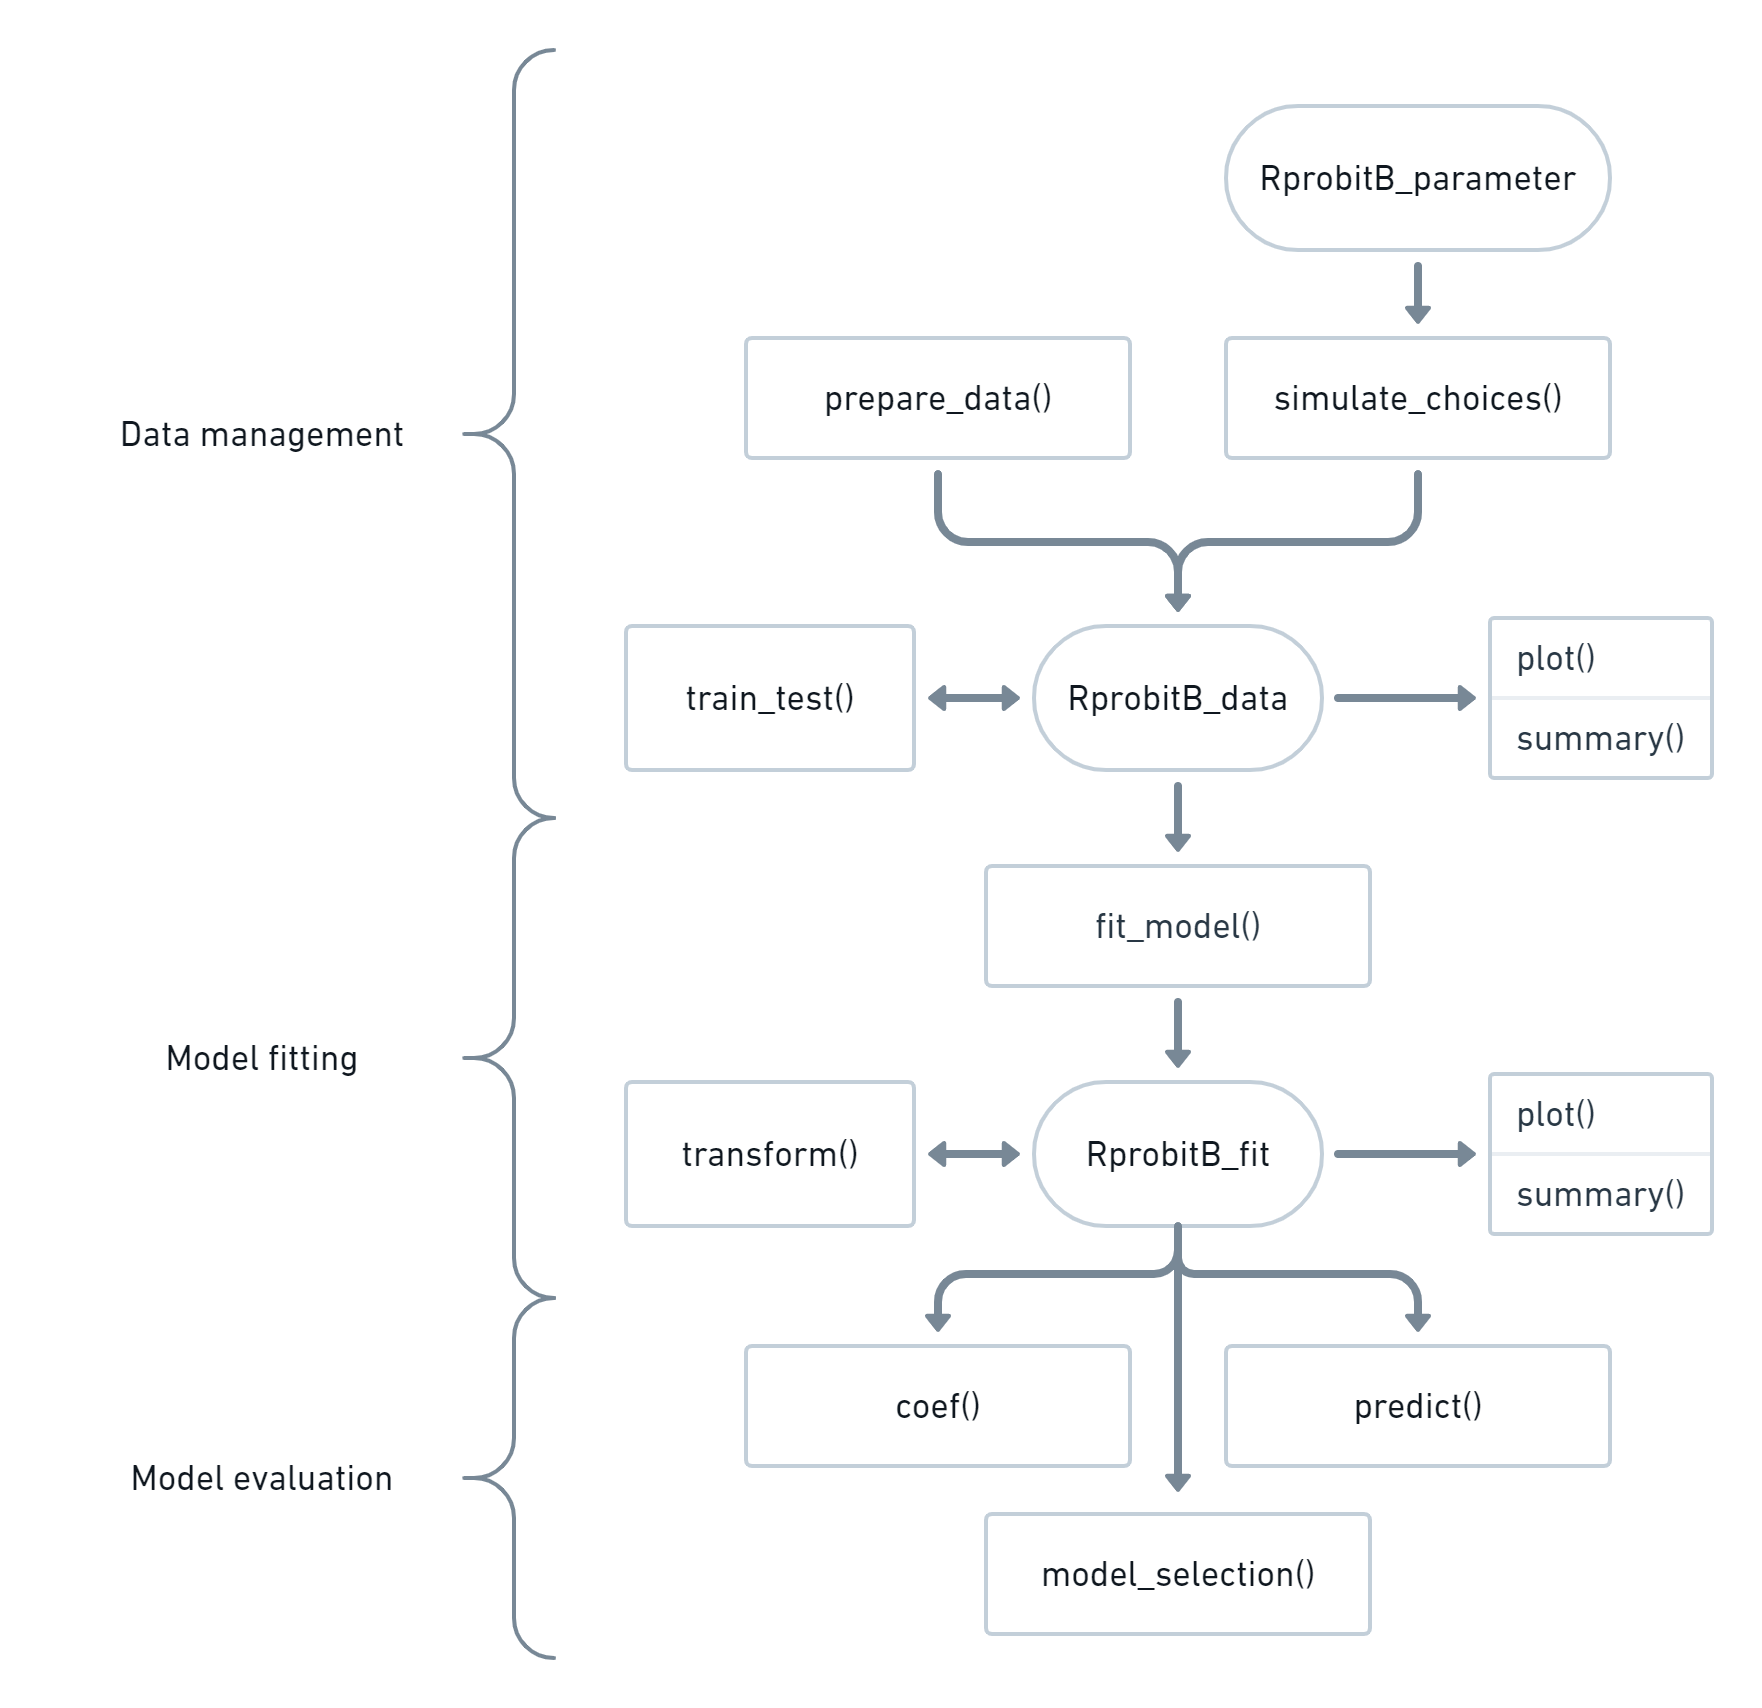
\includegraphics[scale = 0.4]{flowchart.png}
  \caption{Flowchart of the package functionality.}
  \label{fig:flowchart}
\end{figure}


\section{The probit model} \label{sec:probit_model}

The probit model is a regression-type model where the dependent variable only takes a finite number of values and the error term is normally distributed \citep{Agresti:2015}. Its purpose is to estimate the probability that the dependent variable takes a certain, discrete value. The most common application are discrete choice scenarios. The dependent variable here is one of finitely many and mutually exclusive alternatives (that are not ordered), and explanatory variables typically are characteristics of the deciders or the alternatives.

To be concrete, assume that we possess data of $N$ decision makers which choose between $J \geq 2$ alternatives at each of $T$ choice occasions. For notational simplicity, the number of choice occasions $T$ is assumed to be the same for each decision maker here. However, we are not restricted to this case: \pkg{RprobitB} allows for unbalanced panels, i.e. varying $T$. Of course, the cross-sectional case $T = 1$ is possible. Specific to each decision maker, alternative and choice occasion, we furthermore observe $P$ choice attributes that we use to explain the choices. The continuous choice attributes cannot be linked directly to the discrete choices but must take a detour over a latent variable. In the discrete choice setting, this variable can be interpreted as the decider's utility of a certain alternative. Decider $n$'s utility $U_{ntj}$ for alternative $j$ at choice occasion $t$ is modeled as

\begin{equation}
  U_{ntj} = X_{ntj}'\beta + \epsilon_{ntj}
\end{equation}

for $n=1,\dots,N$, $t=1,\dots,T$ and $j=1,\dots,J$, where

- $X_{ntj}$ is a (column) vector of $P$ characteristics of $j$ as faced by $n$ at $t$,

- $\beta \in {\mathbb R}^{P}$ is a vector of coefficients,

- and $(\epsilon_{nt:}) = (\epsilon_{nt1},\dots,\epsilon_{ntJ})' \sim \text{MVN}_{J} (0,\Sigma)$ is the model's error term vector for $n$ at $t$, which in the probit model is assumed to be multivariate normally distributed with zero mean and covariance matrix $\Sigma$.

Now let $y_{nt}=j$ denote the event that decision maker $n$ chooses alternative $j$ at choice occasion $t$. Assuming utility maximizing behavior of the decision makers, the decisions are linked to the utilities via

\begin{equation}
y_{nt} = {\arg \max}_{j = 1,\dots,J} U_{ntj}.
\end{equation}

\subsection{Modeling choice behavior heterogeneity} \label{subsec:heterogeneity}

Note that the coefficient vector $\beta$ in the above definition is constant across decision makers. This assumption is too restrictive for many applications. For example, consider the case of modeling the choice of a means of transportation to work: It is easily imaginable that business people and pensioners do not share the same sensitivities towards cost and time. Heterogeneity in choice behavior can be modeled by imposing a distribution on $\beta$ such that each decider can have their own preferences.

Formally, we define $\beta = (\alpha, \beta_n)$, where $\alpha$ are $P_f$ coefficients that are constant across deciders and $\beta_n$ are $P_r$ decider-specific coefficients. Consequently, $P = P_f + P_r$. Now if $P_r>0$, $\beta_n$ is distributed according to some $P_r$-variate distribution, the so-called mixing distribution.

Choosing an appropriate mixing distribution is a notoriously difficult task of the model specification. In many applications, different types of standard parametric distributions (including the normal, log-normal, uniform and tent distribution) are tried in conjunction with a likelihood value-based model selection, cf. \cite{Train:2009}, Chapter 6. Instead, \pkg{RprobitB} implements the approach of \cite{Oelschlaeger:2020} to approximate any underlying mixing distribution by a mixture of (multivariate) Gaussian densities. More precisely, the underlying mixing distribution $g_{P_r}$ for the random coefficients $(\beta_n)_{n}$ is approximated by a mixture of $P_r$-variate normal densities $\phi_{P_r}$ with mean vectors $b=(b_c)_{c}$ and covariance matrices $\Omega=(\Omega_c)_{c}$ using $C$ components, i.e.

\begin{equation}
\beta_n\mid b,\Omega \sim \sum_{c=1}^{C} s_c \phi_{P_r} (\cdot \mid b_c,\Omega_c).
\end{equation}

Here, $(s_c)_{c}$ are weights satisfying $0 < s_c\leq 1$ for $c=1,\dots,C$ and $\sum_c s_c=1$. One interpretation of the latent class model is obtained by introducing variables $z=(z_n)_n$, allocating each decision maker $n$ to class $c$ with probability $s_c$, i.e.

\begin{equation}
\text{Prob}(z_n=c)=s_c \land \beta_n \mid z,b,\Omega \sim \phi_{P_r}(\cdot \mid b_{z_n},\Omega_{z_n}).
\end{equation}

We call the resulting model the *latent class mixed multinomial probit model*. Note that the model collapses to the *(normally) mixed multinomial probit model* if $P_r>0$ and $C=1$, to the *multinomial probit model* if $P_r=0$ and to the *binary probit model* if additionally $J=2$.

\subsection{Model normalization} \label{subsec:normalization}

As is well known, any utility model needs to be normalized with respect to level and scale in order to be identified \citep{Train:2009}. Therefore, we consider the transformed model

\begin{equation}
\tilde{U}_{ntj} = \tilde{X}_{ntj}' \beta + \tilde{\epsilon}_{ntj},
\end{equation}

$n=1,\dots,N$, $t=1,\dots,T$ and $j=1,\dots,J-1$, where (choosing $J$ as the reference alternative) $\tilde{U}_{ntj} = U_{ntj} - U_{ntJ}$, $\tilde{X}_{ntj} = X_{ntj} - X_{ntJ}$, and $\tilde{\epsilon}_{ntj} = \epsilon_{ntj} - \epsilon_{ntJ}$, where $(\tilde{\epsilon}_{nt:}) = (\tilde{\epsilon}_{nt1},...,\tilde{\epsilon}_{nt(J-1)})'  \sim \text{MVN}_{J-1} (0,\tilde{\Sigma})$ and $\tilde{\Sigma}$ denotes a covariance matrix with the top-left element restricted to one. \pkg{RprobitB} provides an alternative to fixing an error term variance in order to normalize with respect to scale by fixing an element of $\alpha$.

\section{Choice data} \label{sec:choice_data}

\pkg{RprobitB} helps in modeling the choice of individual deciders of one alternative from a finite set of choice alternatives. This choice set has to fulfill three properties \citep{Train:2009}: Choices need to be

1. mutually exclusive (one can choose one and only one alternative that are all different),

2. exhaustive (the alternatives do not leave other options open),

3. and finitely many.

In \pkg{RprobitB} only unordered alternatives (that is, alternatives cannot be ranked) are modeled. Every decider may take one or repeated choices (called choice occasions).

The data set thus contains information on

1. an identifier for each decider (and optionally for each choice situation),

2. the choices,

3. alternative and decider specific covariates.

Additionally, \pkg{RprobitB} asks the following formal requirements:

1. The data set must be in "wide" format, that means each row provides the full information for one choice occasion.

2. It must contain a column with unique identifiers for each decision maker. Additionally, it can contain a column with identifier for each choice situation of each decider. If this information is missing, these identifier are generated automatically by the appearance of the choices in the data set.

3. It can contain a column with the observed choices. Such a column is required for model fitting but not for prediction.

4. It must contain columns for the values of each alternative specific covariate for each alternative and for each decider specific covariate.

\subsection{Model formula} \label{subsec:model_formula}

We have to inform \pkg{RprobitB} about the covariates we want to include in our model via specifying a \code{formula} object. Say we want to model the utility $U_{n,t,j}$ of decider $n$ at choice occasion $t$ for alternative $j$ via the linear equation

$$U_{n,t,j} = A_{n,t,j} \beta_1 + B_{n,t} \beta_{2,j} + C_{n,t,j} \beta_{3,j} + \epsilon_{n,tj}.$$

Here, $A$ and $C$ are alternative and choice situation specific covariates, whereas $B$ is choice situation specific. The coefficient $\beta_1$ is generic (i.e. the same for each alternative), whereas $\beta_{2,j}$ and $\beta_{3,j}$ are alternative specific.

To represent this structure, the `formula` object is of the form (analogously to {mlogit}) `choice ~ A | B | C`, where

- `choice` is the dependent variable (the discrete choice we aim to explain),

- `A` are alternative and choice situation specific covariates with a generic coefficient (we call them covariates of type 1),

- `B` are choice situation specific covariates with alternative specific coefficients. Mind that not all alternative specific coefficients of type 2-covariates are identified. This is because the probit model is estimated on utility differences since the level of the utility is irrelevant, see the vignette on the model definition. Therefore, the coefficient of the last alternative of each type 2-covariate is set to 0. (we call them covariates of type 2),

- and `C` are alternative and choice situation specific covariates with
alternative specific coefficients (we call them covariates of type 3).

Specifying a `formula` object for {RprobitB} must be consistent with the following rules:

- By default, alternative specific constants (ASCs) ASCs capture the average effect on utility of all factors that are not included in the model. Due to identifiability, we cannot estimate ASCs for all the alternatives. Therefore, they are added for all except for the last alternative. are added to the model. They can be removed by adding `+ 0` in the second spot, e.g. `choice ~ A | B + 0 | C`.

- To exclude covariates of the backmost categories, use either `0`, e.g. `choice ~ A | B | 0` or just leave this part out and write `choice ~ A | B `. However, to exclude covariates of front categories, we have to use `0`, e.g. `choice ~ 0 | B`.

- To include more than one covariate of the same category, use `+`, e.g. `choice ~ A1 + A2 | B`.

- If we don't want to include any covariates of the second category but we want to estimate alternative specific constants, add `1` in the second spot, e.g. `choice ~ A | 1`. The expression `choice ~ A | 0` is interpreted as no covariates of the second category and no alternative specific constants.

To impose random effects for specific variables, we need to define a character vector `re` with the corresponding variable names. To have random effects for the alternative specific constants, include `"ASC"` in `re`.

\subsection{The prepare data function} \label{subsec:prepare_data}

Before model estimation with \pkg{RprobitB}, any empirical choice data set \code{choice_data} must pass the \fct{prepare\_data} function:

\begin{Schunk}
\begin{Sinput}
> data <- prepare_data(form = form, choice_data = choice_data)
\end{Sinput}
\end{Schunk}

The function performs compatibility checks and data transformations and returns an object of class \class{RprobitB\_data} that can be fed into the estimation routine \fct{mcmc}. The following arguments are optional:

- \code{re}: The character vector of variable names of \code{form} with random effects. \code{re = NULL} per default, i.e. no random effects.

- \code{alternatives}: We may not want to consider all alternatives in \code{choice_data}. In that case, we can specify a character vector \code{alternatives} with selected names of alternatives. If not specified, the choice set is defined by the observed choices.

- \code{id}: A character (single string), the name of the column in \code{choice_data} that contains a unique identifier for each decision maker. The default is \code{"id"}.

- \code{idc}: A character, the name of the column in \code{choice_data} that contains a unique identifier for each choice situation given the decision maker. Per default, these identifier are generated by the appearance of the choices in the data set.

- \code{standardize}: A character vector of variable names of `form` that get standardized. Covariates of type 1 or 3 have to be addressed by \code{<covariate>_<alternative>}. If \code{standardize = "all"}, all covariates get standardized. Per default, no covariate is standardized.

- \code{impute}: Specifies how to handle missing entries (\code{NA, NaN, -Inf, Inf}) in \code{choice_data}. The following options are available:

  - \code{"complete_cases"}, which removes rows containing missing entries (the default),

  - \code{"zero_out"}, which replaces missing entries by zero,

  - \code{"mean"}, which imputes missing entries by the covariate mean.

\subsection{Example 1: Train data} \label{subsec:train_data_prep}

The Train data set contains 2929 stated choices by 235 Dutch individuals deciding between two virtual train trip options based on the price, the travel time, the level of comfort, and the number of changes. It fulfills the above requirements: Each row represents one choice occasion, the columns `id` and `choiceid` identify the deciders and the choice occasions, respectively. The column `choice` gives the observed choices. Four alternative-specific covariates are available, namely `price`, `time`, `change`, and `comfort`. There values are given for each alternative. For alternative specific variables, the alternative names must be added to the covariates via the \code{\_} separator.

\begin{Schunk}
\begin{Sinput}
> data("Train", package = "mlogit")
> str(Train)
\end{Sinput}
\begin{Soutput}
'data.frame':	2929 obs. of  11 variables:
 $ id       : int  1 1 1 1 1 1 1 1 1 1 ...
 $ choiceid : int  1 2 3 4 5 6 7 8 9 10 ...
 $ choice   : Factor w/ 2 levels "A","B": 1 1 1 2 2 2 2 2 1 1 ...
 $ price_A  : num  2400 2400 2400 4000 2400 4000 2400 2400 4000 2400 ...
 $ time_A   : num  150 150 115 130 150 115 150 115 115 150 ...
 $ change_A : num  0 0 0 0 0 0 0 0 0 0 ...
 $ comfort_A: num  1 1 1 1 1 0 1 1 0 1 ...
 $ price_B  : num  4000 3200 4000 3200 3200 2400 3200 3200 3200 4000 ...
 $ time_B   : num  150 130 115 150 150 130 115 150 130 115 ...
 $ change_B : num  0 0 0 0 0 0 0 0 0 0 ...
 $ comfort_B: num  1 1 0 0 0 0 1 0 1 0 ...
\end{Soutput}
\end{Schunk}

We specify a model formula for the Train data set. Say we want to include all the covariates \code{price}, \code{time}, \code{comfort}, and \code{change}, which are all alternative specific (that is, they contain a potentially different value for each alternative, such as different prices for A and B), so either of type 1 or type 3. The difference between type 1 and type 3 is that in the former case, we would estimate a generic coefficient (i.e. a coefficient that is constant across alternatives), whereas in the latter case, we would estimate alternative specific coefficients. Deciding between type 1 and type 3 for these covariates belongs into the topic of model selection, for which we provide a separate vignette. For now, we go with type 1 for all covariates and remove ASCs:

\begin{Schunk}
\begin{Sinput}
> form <- choice ~ price + time + comfort + change | 0
\end{Sinput}
\end{Schunk}

Additionally, we specify random effects for \code{price} and \code{time} (because we would typically expect heterogeneity here):

\begin{Schunk}
\begin{Sinput}
> re <- c("price","time")
\end{Sinput}
\end{Schunk}

\pkg{RprobitB} provides the function \fct{check\_form} which can be used to check if \code{form} and \code{re} are correctly interpreted:

\begin{Schunk}
\begin{Sinput}
> check_form(form = form, re = re)
\end{Sinput}
\begin{Soutput}
choice ~ price + time + comfort + change | 0
- dependent variable: choice 
- type 1 covariate(s): price, time, comfort, change 
- type 2 covariate(s):  
- type 3 covariate(s):  
- random effects: price, time 
- ASC: FALSE 
\end{Soutput}
\end{Schunk}

Let's prepare the Train data set for estimation with our previous specification of \code{form} and \code{re}:

\begin{Schunk}
\begin{Sinput}
> data <- prepare_data(form = form, choice_data = Train, re = re, id = "id", idc = "choiceid")
\end{Sinput}
\end{Schunk}

The \fct{summary} and \fct{plot} methods provide a quick data overview:

\begin{Schunk}
\begin{Sinput}
> summary(data)
\end{Sinput}
\begin{Soutput}
Summary of empirical choice data
235 decision makers 
5 to 19 choice occasions each 
2929 choices in total

Alternatives
  frequency
A      1474
B      1455

Linear coefficients
     name    re
1 comfort FALSE
2  change FALSE
3   price  TRUE
4    time  TRUE
\end{Soutput}
\begin{Sinput}
> plot(data)
\end{Sinput}
\end{Schunk}
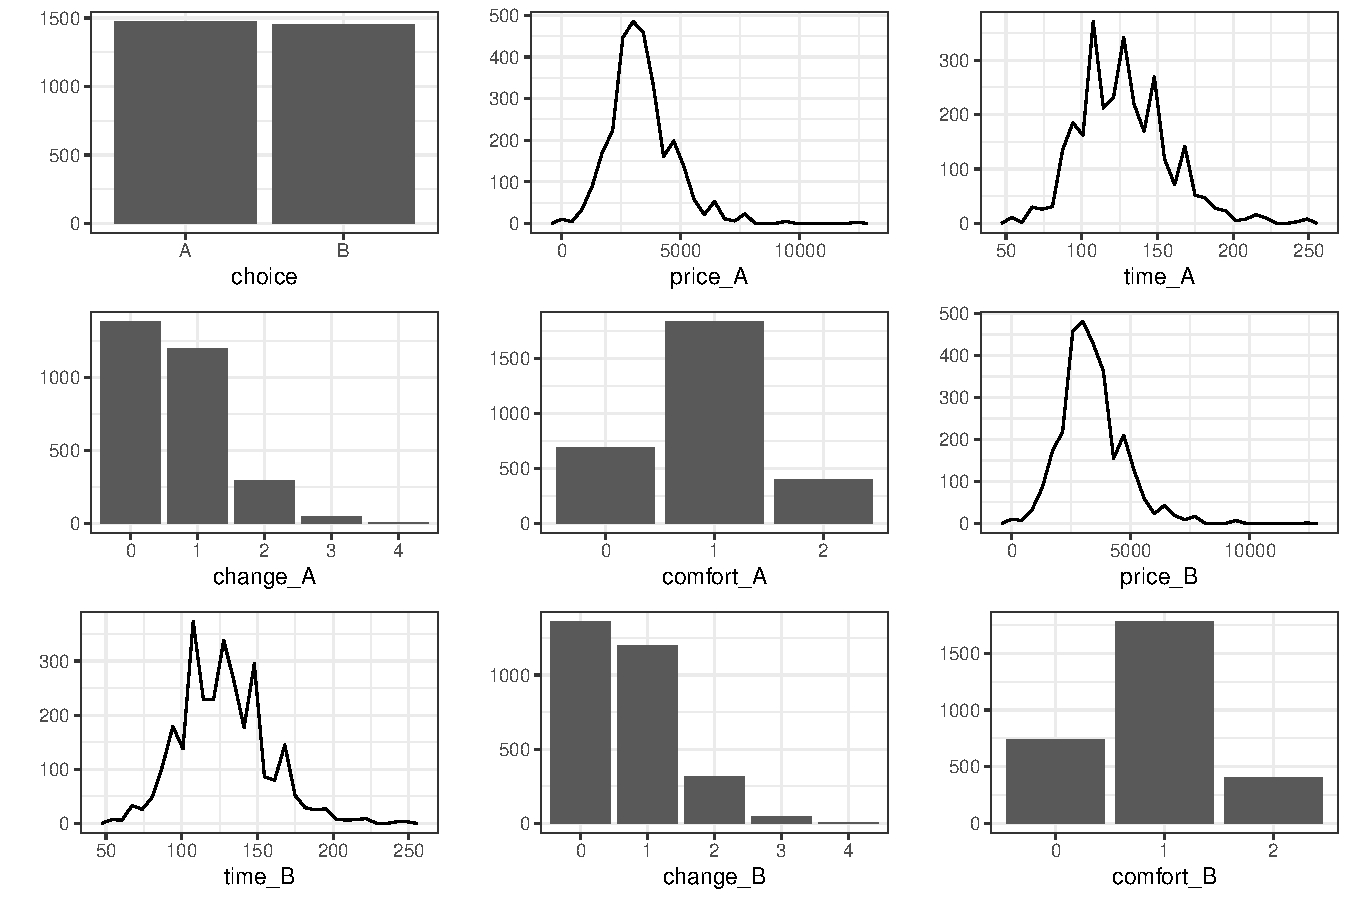
\includegraphics{rprobitb_oelschlaeger_bauer-summary-plot-Train-data}

\subsection{Simulate choices} \label{subsec:simulate_choices}

The \fct{simulate\_choices} function simulates discrete choice data from a prespecified probit model. Say we want to simulate the choices of \code{N} deciders in \code{T} choice occasions (\code{T} can be either a positive number, representing a fixed number of choice occasions for each decision maker, or a vector of length \code{N} with decision maker specific numbers of choice occasions) among \code{J} alternatives from a model formulation \code{form}, we have to call

\begin{Schunk}
\begin{Sinput}
> data <- simulate_choices(form = form, N = N, T = T, J = J)
\end{Sinput}
\end{Schunk}

The function \fct{simulate\_choices} has the following optional arguments:

- \code{re}: The character vector of variable names of \code{form} with random effects.

- \code{alternatives}: A character vector of length \code{J} with the names of the choice alternatives. If not specified, the alternatives are labeled by the first \code{J} upper-case letters of the Roman alphabet.

- \code{covariates}: A named list of covariate values. Each element must be a vector of length equal to the number of choice occasions and named according to a covariate, or follow the naming convention for alternative specific covariates, i.e. \code{<covariate>\_<alternative>}. Covariates for which no values are specified are drawn from a standard normal distribution.

- \code{standardize}: A character vector of variable names of \code{form} that get standardized.

- \code{seed}: Set a seed for the simulation.

We can specify the true parameters by adding values for

- \code{alpha}, the fixed coefficient vector,

- \code{C}, the number (greater or equal 1) of latent classes of decision makers,

- \code{s}, the vector of class weights,

- \code{b}, the matrix of class means as columns,

- \code{Omega}, the matrix of class covariance matrices as columns,

- \code{Sigma}, the differenced error term covariance matrix, or \code{Sigma\_full}, the full error term covariance matrix,

- \code{beta}, the matrix of the decision-maker specific coefficient vectors,

- \code{z}, the class allocation vector.

True parameters that are not specified will be set at random.

\subsection{Example 2: Simulated choices} \label{subsec:example_simulated_choices}

For illustration, we simulate the choices of \code{N = 100} deciders at \code{T = 10} choice occasions between the alternatives \code{A} and \code{B}:

\begin{Schunk}
\begin{Sinput}
> N <- 100
> T <- 10
> alternatives <- c("A", "B")
> form <- choice ~ var1 | var2 | var3
> re <- c("ASC", "var2")
\end{Sinput}
\end{Schunk}

\pkg{RprobitB} provides the function \fct{overview\_effects} which can be used to get an overview of the effects for which parameters can be specified:

\begin{Schunk}
\begin{Sinput}
> overview_effects(form = form, re = re, alternatives = alternatives)
\end{Sinput}
\begin{Soutput}
    name    re
1   var1 FALSE
2 var3_A FALSE
3 var3_B FALSE
4 var2_A  TRUE
5  ASC_A  TRUE
\end{Soutput}
\end{Schunk}

Hence, the coefficient vector \code{alpha} must be of length 3, where the elements 1 to 3 correspond to \code{var1}, \code{var3\_A}, and \code{var3\_B}, respectively. The matrix \code{b} must be of dimension \code{2 x C}, where (by default) \code{C = 1} and row 1 and 2 correspond to \code{var2\_A} and \code{ASC\_A}, respectively.

\begin{Schunk}
\begin{Sinput}
> data <- simulate_choices(
+    form = form,
+    N = N,
+    T = T,
+    J = 2,
+    re = re,
+    alternatives = alternatives,
+    seed = 1,
+    alpha = c(-1,0,1),
+    b = matrix(c(2,-0.5), ncol = 1)
+  )
> summary(data)
\end{Sinput}
\begin{Soutput}
Summary of simulated choice data
100 decision makers 
10 choice occasions each 
1000 choices in total

Alternatives
  frequency
A       489
B       511

Linear coefficients
    name    re
1   var1 FALSE
2 var3_A FALSE
3 var3_B FALSE
4 var2_A  TRUE
5  ASC_A  TRUE
\end{Soutput}
\end{Schunk}

We can visualize the covariates grouped by the chosen alternatives:

\begin{Schunk}
\begin{Sinput}
> plot(data, by_choice = TRUE)
\end{Sinput}
\end{Schunk}
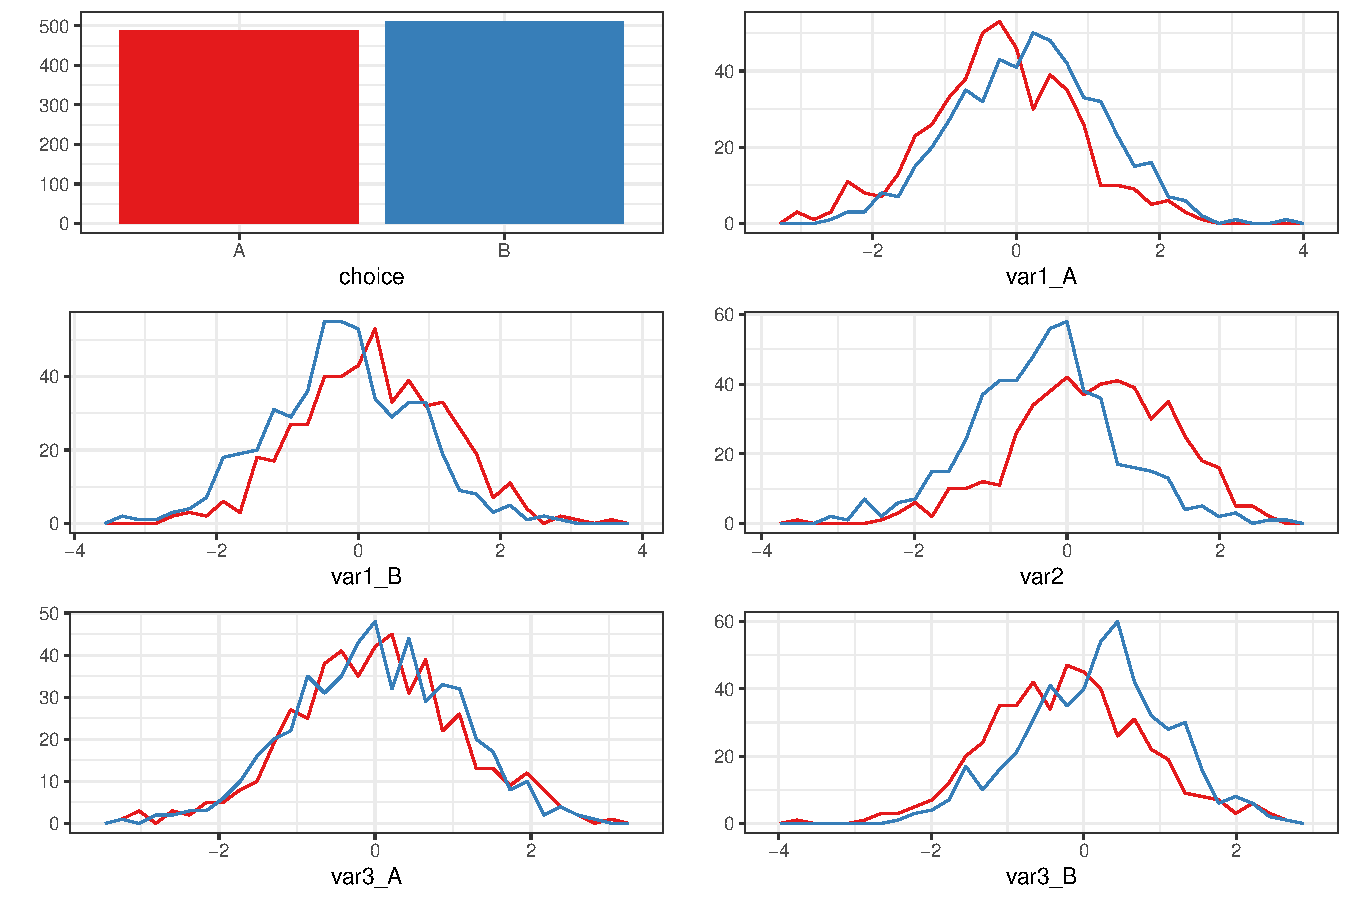
\includegraphics{rprobitb_oelschlaeger_bauer-data-sim-plot-by-choice}

What we see is consistent with our specification: Higher values of \code{var1\_A} for example correspond more frequently to choice \code{B} (upper-right panel), because the coefficient of \code{var1} (the first value of \code{alpha}) is negative.

\subsection{Train and test data set} \label{subsec:train_test}

The function \fct{train\_test} can be used to split the output of \fct{prepare\_data} or \fct{simulate\_choices} into a train and a test subset. This is useful when evaluating the prediction performance of a fitted model. For example, the following code puts 70\% of deciders from our simulated \code{data} into the train subsample and 30\% of deciders in the test subsample:

\begin{Schunk}
\begin{Sinput}
> train_test(data, test_proportion = 0.3, by = "N")
\end{Sinput}
\begin{Soutput}
$train
Simulated data of 700 choices.

$test
Simulated data of 300 choices.
\end{Soutput}
\end{Schunk}

Alternatively, the following code puts 2 randomly chosen choice occasions per decider from \code{data} into the test subsample, the rest goes into the train subsample:

\begin{Schunk}
\begin{Sinput}
> train_test(data, test_number = 2, by = "T", random = TRUE, seed = 1)
\end{Sinput}
\begin{Soutput}
$train
Simulated data of 800 choices.

$test
Simulated data of 200 choices.
\end{Soutput}
\end{Schunk}

\section{Model fitting} \label{sec:model_fitting}

Bayes estimation of the probit model builds upon the work of \cite{McCulloch:1994}, \cite{Nobile:1998}, \cite{Allenby:1998}, and \cite{Imai:2005}. A key ingredient is the concept of data augmentation, see \cite{Albert:1993}: The idea is to treat the latent utilities $U$ in the model equation $U = X\beta + \epsilon$ as additional parameters. Then, conditional on $U$, the probit model constitutes a standard Bayesian linear regression set-up. Its posterior distribution can be approximated by iteratively drawing and updating each model parameter conditional on the other parameters (the so-called Gibbs sampling approach).

A priori, we assume the following (conjugate) parameter distributions:

- $(s_1,\dots,s_C)\sim D_C(\delta)$, where $D_C(\delta)$ denotes the $C$-dimensional Dirichlet distribution with concentration parameter vector $\delta = (\delta_1,\dots,\delta_C)$,

- $\alpha\sim \text{MVN}_{P_f}(\psi,\Psi)$, where $\text{MVN}_{P_f}$ denotes the $P_f$-dimensional normal distribution with mean $\psi$ and covariance $\Psi$,

- $b_c \sim \text{MVN}_{P_r}(\xi,\Xi)$, independent for all $c$,

- $\Omega_c \sim W^{-1}_{P_r}(\nu,\Theta)$, independent for all $c$, where $W^{-1}_{P_r}(\nu,\Theta)$ denotes the $P_r$-dimensional inverse Wishart distribution with $\nu$ degrees of freedom and scale matrix $\Theta$,

- and $\Sigma \sim W^{-1}_{J-1}(\kappa,\Lambda)$.

These prior distributions imply the following conditional posterior distributions:

- The class weights are drawn from the Dirichlet distribution
\begin{equation}
(s_1,\dots,s_C)\mid \delta,z \sim D_C(\delta_1+m_1,\dots,\delta_C+m_C),
\end{equation}
where for $c=1,\dots,C$, $m_c=\#\{n:z_n=c\}$ denotes the current absolute class size. Mind that the model is invariant to permutations of the class labels $1,\dots,C$. For that reason, we accept an update only if the ordering $s_1>\dots>s_C$ holds, thereby ensuring a unique labeling of the classes.

- Independently for all $n$, we update the allocation variables $(z_n)_n$ from their conditional distribution
\begin{equation}
\text{Prob}(z_n=c\mid s,\beta,b,\Omega )=\frac{s_c\phi_{P_r}(\beta_n\mid b_c,\Omega_c)}{\sum_c s_c\phi_{P_r}(\beta_n\mid b_c,\Omega_c)}.
\end{equation}

- The class means $(b_c)_c$ are updated independently for all $c$ via
\begin{equation}
b_c\mid \Xi,\Omega,\xi,z,\beta \sim\text{MVN}_{P_r}\left( \mu_{b_c}, \Sigma_{b_c}  \right),
\end{equation}
where $\mu_{b_c}=(\Xi^{-1}+m_c\Omega_c^{-1})^{-1}(\Xi^{-1}\xi +m_c\Omega_c^{-1}\bar{b}_c)$, $\Sigma_{b_c}=(\Xi^{-1}+m_c\Omega_c^{-1})^{-1}$, $\bar{b}_c=m_c^{-1}\sum_{n:z_n=c} \beta_n$.

- The class covariance matrices $(\Omega_c)_c$ are updated independently for all $c$ via
\begin{equation}
\Omega_c \mid \nu,\Theta,z,\beta,b \sim W^{-1}_{P_r}(\mu_{\Omega_c},\Sigma_{\Omega_c}),
\end{equation}
where $\mu_{\Omega_c}=\nu+m_c$ and $\Sigma_{\Omega_c}=\Theta^{-1} + \sum_{n:z_n=c} (\beta_n-b_c)(\beta_n-b_c)'$.

- Independently for all $n$ and $t$ and conditionally on the other components, the utility vectors $(U_{nt:})$ follow a $J-1$-dimensional truncated multivariate normal distribution, where the truncation points are determined by the choices $y_{nt}$. To sample from a truncated multivariate normal distribution, we apply a sub-Gibbs sampler, following the approach of \cite{Geweke:1998}:
\begin{equation}
U_{ntj} \mid U_{nt(-j)},y_{nt},\Sigma,W,\alpha,X,\beta
\sim \mathcal{N}(\mu_{U_{ntj}},\Sigma_{U_{ntj}}) \cdot \begin{cases}
1(U_{ntj}>\max(U_{nt(-j)},0) ) & \text{if}~ y_{nt}=j\\
1(U_{ntj}<\max(U_{nt(-j)},0) ) & \text{if}~ y_{nt}\neq j
\end{cases},
\end{equation}
where $U_{nt(-j)}$ denotes the vector $(U_{nt:})$ without the element $U_{ntj}$, $\mathcal{N}$ denotes the univariate normal distribution, $\Sigma_{U_{ntj}} = 1/(\Sigma^{-1})_{jj}$ and
\begin{equation}
\mu_{U_{ntj}} = W_{ntj}'\alpha + X_{ntj}'\beta_n - \Sigma_{U_{ntj}} (\Sigma^{-1})_{j(-j)}   (U_{nt(-j)} - W_{nt(-j)}'\alpha - X_{nt(-j)}' \beta_n ),
\end{equation}
where $(\Sigma^{-1})_{jj}$ denotes the $(j,j)$th element of $\Sigma^{-1}$, $(\Sigma^{-1})_{j(-j)}$ the $j$th row without the $j$th entry, $W_{nt(-j)}$ and $X_{nt(-j)}$ the coefficient matrices $W_{nt}$ and $X_{nt}$, respectively, without the $j$th column.

- Updating the fixed coefficient vector $\alpha$ is achieved by applying the formula for Bayesian linear regression of the regressors $W_{nt}$ on the regressands $(U_{nt:})-X_{nt}'\beta_n$, i.e.
\begin{equation}
\alpha \mid \Psi,\psi,W,\Sigma,U,X,\beta \sim \text{MVN}_{P_f}(\mu_\alpha,\Sigma_\alpha),
\end{equation}
where $\mu_\alpha = \Sigma_\alpha (\Psi^{-1}\psi + \sum_{n=1,t=1}^{N,T} W_{nt} \Sigma^{-1} ((U_{nt:})-X_{nt}'\beta_n) )$ and $\Sigma_\alpha = (\Psi^{-1} + \sum_{n=1,t=1}^{N,T} W_{nt}\Sigma^{-1} W_{nt}^{'} )^{-1}$.

- Analogously to $\alpha$, the random coefficients $(\beta_n)_n$ are updated independently via
\begin{equation}
\beta_n \mid \Omega,b,X,\Sigma,U,W,\alpha \sim \text{MVN}_{P_r}(\mu_{\beta_n},\Sigma_{\beta_n}),
\end{equation}
where $\mu_{\beta_n} = \Sigma_{\beta_n} (\Omega_{z_n}^{-1}b_{z_n} + \sum_{t=1}^{T} X_{nt} \Sigma^{-1} (U_{nt}-W_{nt}'\alpha) )$ and $\Sigma_{\beta_n} = (\Omega_{z_n}^{-1} + \sum_{t=1}^{T} X_{nt}\Sigma^{-1} X_{nt}^{'} )^{-1}$ .

- The error term covariance matrix $\Sigma$ is updated by means of
\begin{equation}
\Sigma \mid \kappa,\Lambda,U,W,\alpha,X,\beta \sim W^{-1}_{J-1}(\kappa+NT,\Lambda+S), \\
\end{equation}
where $S = \sum_{n=1,t=1}^{N,T} \varepsilon_{nt} \varepsilon_{nt}'$ and $\varepsilon_{nt} = (U_{nt:}) - W_{nt}'\alpha - X_{nt}'\beta_n$.

\subsection{Parameter normalization} \label{subsec:parameter_normalization}

Samples obtained from the updating scheme described above lack identification (except for $s$ and $z$ draws), compare to the vignette on the model definition. Therefore, subsequent to the sampling, the following normalization is required for the $i$th update in each iteration $i$:

- $\alpha^{(i)} \cdot \omega^{(i)}$,

- $b_c^{(i)} \cdot \omega^{(i)}$, $c=1,\dots,C$,

- $U_{nt}^{(i)} \cdot \omega^{(i)}$, $n = 1,\dots,N$, $t = 1,\dots,T$,

- $\beta_n^{(i)} \cdot \omega^{(i)}$, $n = 1,\dots,N$,

- $\Omega_c^{(i)} \cdot (\omega^{(i)})^2$, $c=1,\dots,C$, and

- $\Sigma^{(i)} \cdot (\omega^{(i)})^2$,

where either $\omega^{(i)} = \sqrt{\text{const} / (\Sigma^{(i)})_{jj}}$ with $(\Sigma^{(i)})_{jj}$ the $j$th diagonal element of $\Sigma^{(i)}$, $1\leq j \leq J-1$, or alternatively $\omega^{(i)} = \text{const} / \alpha^{(i)}_p$ for some coordinate $1\leq p \leq P_f$ of the $i$th draw for the coefficient vector $\alpha$. Here, $\text{const}$ is any positive constant (typically 1). The preferences will be flipped if $\omega^{(i)} < 0$, which only is the case if $\alpha^{(i)}_p < 0$.

\subsection{Burn-in and thinning} \label{subsec:burn_thin}

The theory behind Gibbs sampling constitutes that the sequence of samples produced by the updating scheme is a Markov chain with stationary distribution equal to the desired joint posterior distribution. It takes a certain number of iterations for that stationary distribution to be approximated reasonably well. Therefore, it is common practice to discard the first $B$ out of $R$ samples (the so-called burn-in period). Furthermore, correlation between nearby samples should be expected. In order to obtain independent samples, we consider only every $Q$th sample when computing Gibbs sample statistics like expectation and standard deviation. The independence of the samples can be verified by computing the serial correlation and the convergence of the Gibbs sampler can be checked by considering trace plots, see below.

\subsection{The mcmc function} \label{subsec:mcmc_function}

The Gibbs sampling scheme described above can be executed by applying the function

\begin{Schunk}
\begin{Sinput}
> mcmc(data = data)
\end{Sinput}
\end{Schunk}

where \code{data} must be an \class{RprobitB\_data} object (see the vignette about choice data). The function has the following optional arguments:

- \code{scale}: A named list of three elements, determining the parameter normalization:

  - \code{parameter}: Either \code{"a"} (for an element of \code{alpha}) or \code{"s"} (for a diagonal element of \code{Sigma}). Use the \fct{overview\_effects} function to determine the parameter index. Note that you can set \code{"parameter" = "a"} only if the model has parameters with a fixed coefficient, i.e. only if \code{P\_f>0}.

  - \code{index}: The index of the parameter that gets fixed.

  - \code{value}: The value for the fixed parameter (i.e. the value $\text{const}$ introduced above.

  Per default, the first error-term variance is fixed to 1, i.e. \code{scale = list("parameter" = "s", "index" = 1, "value" = 1)}.

- \code{R}: The number of iterations of the Gibbs sampler. The default is \code{R = 10000}.

- \code{B}: The length of the burn-in period, i.e. a non-negative number of samples to be discarded. The default is \code{B = R/2}.

- \code{Q}: The thinning factor for the Gibbs samples, i.e. only every \code{Q}th sample is kept. The default is \code{Q = 1}.

- \code{print\_progress}: A boolean, determining whether to print the Gibbs sampler progress.

- \code{prior}: A named list of parameters for the prior distributions (their default values are documented in the \fct{check\_prior} function):

  - \code{eta}: The mean vector of length \code{P\_f} of the normal prior for \code{alpha}.

  - \code{Psi}: The covariance matrix of dimension \code{P\_f x P\_f} of the normal prior for \code{alpha}.

  - \code{delta}: The concentration parameter of length 1 of the Dirichlet prior for \code{s}.

  - \code{xi}: The mean vector of length \code{P\_r} of the normal prior for each \code{b\_c}.

  - \code{D}: The covariance matrix of dimension \code{P\_r} x \code{P\_r} of the normal prior for each \code{b\_c}.

  - \code{nu}: The degrees of freedom (a natural number greater than \code{P\_r}) of the Inverse Wishart prior for each \code{Omega\_c}.

  - \code{Theta}: The scale matrix of dimension \code{P\_r} x \code{P\_r} of the Inverse Wishart prior for each \code{Omega\_c}.

  - \code{kappa}: The degrees of freedom (a natural number greater than `J-1`) of the Inverse Wishart prior for \code{Sigma}.

  - \code{E}: The scale matrix of dimension \code{J-1} x \code{J-1} of the Inverse Wishart prior for \code{Sigma}.

- \code{latent\_classes}: A list of parameters specifying the number and the updating scheme of latent classes, see the vignette on modeling heterogeneity fitting.

\subsection{Example 1: Train (cont.)} \label{subsec:train_cont}

In the previous vignette on choice data we introduced the Train data set from the mlogit package \citep{Croissant:2020} that contains 2922 choices between two fictional train route alternatives. First, we transform the travel \code{time} from minutes to hours and the travel \code{price} from guilders to euros:

\begin{Schunk}
\begin{Sinput}
> data("Train", package = "mlogit")
> Train$price_A <- Train$price_A / 100 * 2.20371
> Train$price_B <- Train$price_B / 100 * 2.20371
> Train$time_A <- Train$time_A / 60
> Train$time_B <- Train$time_B / 60
\end{Sinput}
\end{Schunk}

The following lines fit a probit model that explains the chosen trip alternatives (\code{choice}) by their \code{price}, \code{time}, number of \code{change} s, and level of \code{comfort} (the lower this value the higher the comfort). For normalization, the first linear coefficient, the \code{price}, was fixed to \code{-1}, which allows to interpret the other coefficients as monetary values:

\begin{Schunk}
\begin{Sinput}
> form <- choice ~ price + time + change + comfort | 0
> data <- prepare_data(form = form, choice_data = Train)
> model_train <- mcmc(
+    data = data,
+    scale = list("parameter" = "a", index = 1, value = -1)
+  )
\end{Sinput}
\end{Schunk}

The estimated model is saved in \pkg{RprobitB} and can be accessed via

\begin{Schunk}
\begin{Sinput}
> data(model_train, package = "RprobitB")
\end{Sinput}
\end{Schunk}

The estimated coefficients (using the mean of the Gibbs samples as a point estimate) can be printed via

\begin{Schunk}
\begin{Sinput}
> coef(model_train)
\end{Sinput}
\begin{Soutput}
           Estimate   (sd)
1   price     -1.00 (0.00)
2    time    -25.39 (2.23)
3  change     -4.79 (0.86)
4 comfort    -14.40 (0.90)
\end{Soutput}
\end{Schunk}

and visualized via

\begin{Schunk}
\begin{Sinput}
> plot(coef(model_train), sd = 3)
\end{Sinput}
\end{Schunk}
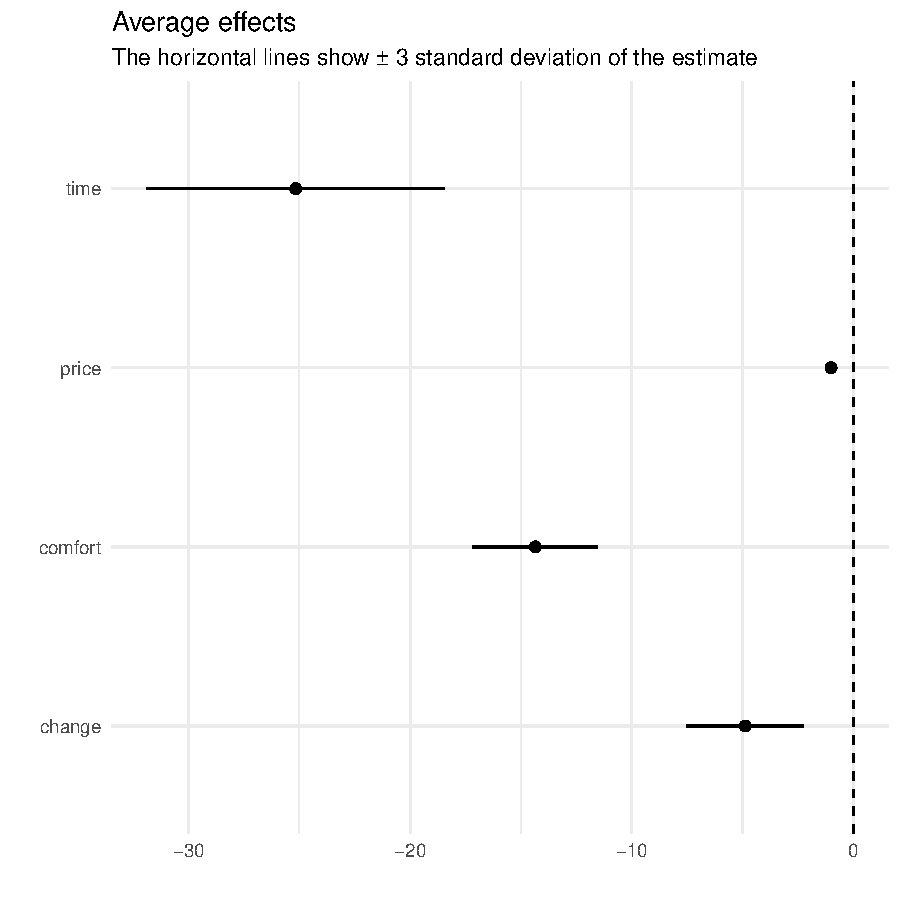
\includegraphics{rprobitb_oelschlaeger_bauer-plot-coef-model-train}

The results indicate that the deciders value one hour travel time by about 25 euros, an additional change by 5 euros, and a more comfortable class by 14 euros. These results are consistent with the ones that are presented in a vignette of the mlogit package on the same data set but using the logit model.

\subsection{Checking the Gibbs samples} \label{subsec:checking-gibbs-samples}

The Gibbs samples are saved in list form in the \class{RprobitB\_fit} object at the entry \code{"gibbs\_samples"}, i.e.

\begin{Schunk}
\begin{Sinput}
> str(model_train$gibbs_samples, max.level = 2, give.attr = FALSE)
\end{Sinput}
\begin{Soutput}
List of 2
 $ gibbs_samples_nbt:List of 2
  ..$ alpha: num [1:500, 1:4] -1 -1 -1 -1 -1 -1 -1 -1 -1 -1 ...
  ..$ Sigma: num [1:500, 1] 607 581 627 615 850 ...
 $ gibbs_samples_raw:List of 2
  ..$ alpha: num [1:10000, 1:4] -0.000739 -0.017192 -0.027834 -0.034068 -0.035992 ...
  ..$ Sigma: num [1:10000, 1] 1.022 0.992 0.941 0.921 0.905 ...
\end{Soutput}
\end{Schunk}

This object contains 2 elements:

- \code{gibbs\_samples\_raw} is a list of the raw samples from the Gibbs sampler,

- and \code{gibbs\_samples\_nbt} are the Gibbs samples used for parameter estimates, i.e. the normalized and thinned Gibbs samples after the burn-in.

Calling the summary function on the estimated \class{RprobitB\_fit} object yields additional information about the Gibbs samples \code{gibbs\_samples\_nbt}. You can specify a list \code{FUN} of functions that compute any point estimate of the Gibbs samples (Use the function \fct{point\_estimates} to access the Gibbs sample statistics as an \class{RprobitB\_parameter} object), for example

- \fct{mean} for the arithmetic mean,

- \fct{stats::sd} for the standard deviation,

- \fct{R\_hat} for the Gelman-Rubin statistic \citep{Gelman:1992} (A Gelman-Rubin statistic close to 1 indicates that the chain of Gibbs samples converged to the stationary distribution),

- or custom statistics like the absolute difference between the median and the mean.

\begin{Schunk}
\begin{Sinput}
> summary(model_train,
+          FUN = c("mean"        = mean,
+                  "sd"          = stats::sd,
+                  "R^"          = R_hat,
+                  "custom_stat" = function(x) abs(mean(x) - median(x))
+                  )
+         )
\end{Sinput}
\begin{Soutput}
Probit model
choice ~ price + time + change + comfort | 0 
R: 10000 
B: 5000 
Q: 10 

Normalization
Level: Utility differences with respect to alternative 2.
Scale: Coefficient of alpha_1 fixed to -1.

Gibbs sample statistics
               mean           sd           R^  custom_stat
 alpha
                                                          
     1        -1.00         0.00         1.00         0.00
     2       -25.39         2.23         1.01         0.00
     3        -4.79         0.86         1.00         0.02
     4       -14.40         0.90         1.00         0.01

 Sigma
                                                          
   1,1       658.58        62.47         1.00         6.38
\end{Soutput}
\end{Schunk}

Calling the \fct{plot} method with the additional argument \code{type = "trace"} plots the trace of the Gibbs samples \code{gibbs\_samples\_nbt}:

\begin{Schunk}
\begin{Sinput}
> par(mfrow = c(2,1))
> plot(model_train, type = "trace")
\end{Sinput}
\end{Schunk}
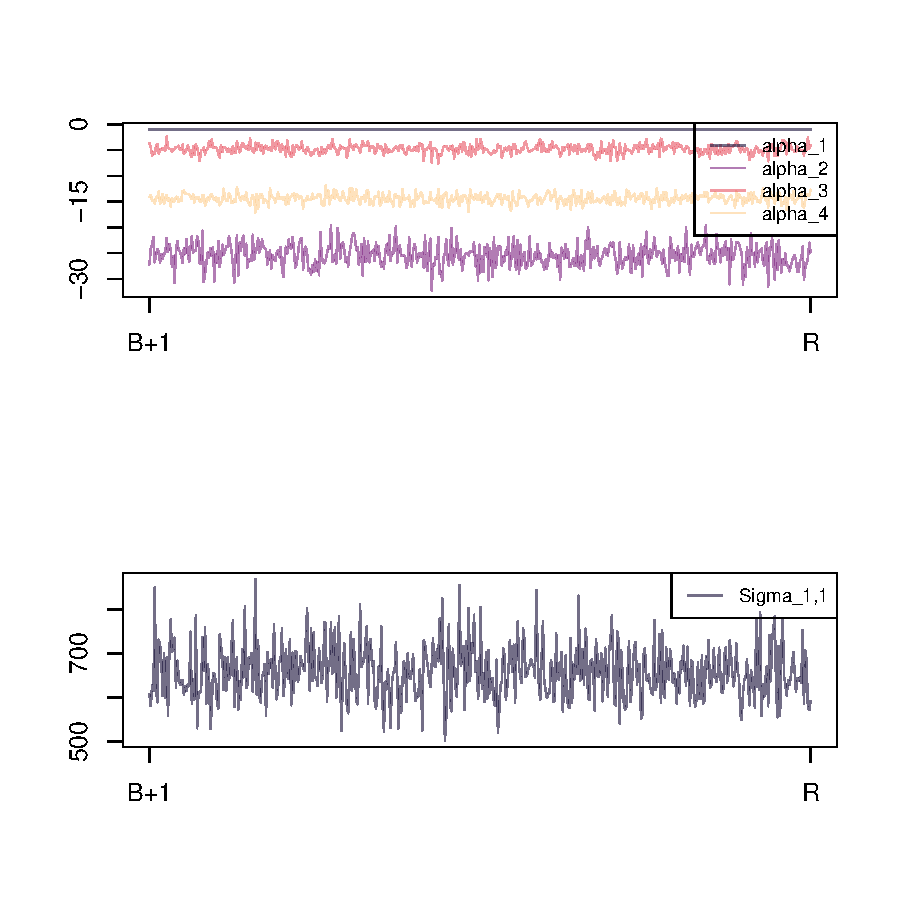
\includegraphics{rprobitb_oelschlaeger_bauer-plot-trace-model-train}

Additionally, we can visualize the serial correlation of the Gibbs samples via the argument \code{type = "acf"}. The boxes in the top-right corner state the total sample size TSS (here \code{R} - \code{B} = 10000 - 5000 = 5000), the effective sample size ESS, and the factor by which TSS is larger than ESS.

\begin{Schunk}
\begin{Sinput}
> par(mfrow = c(2,3))
> plot(model_train, type = "acf")
\end{Sinput}
\end{Schunk}
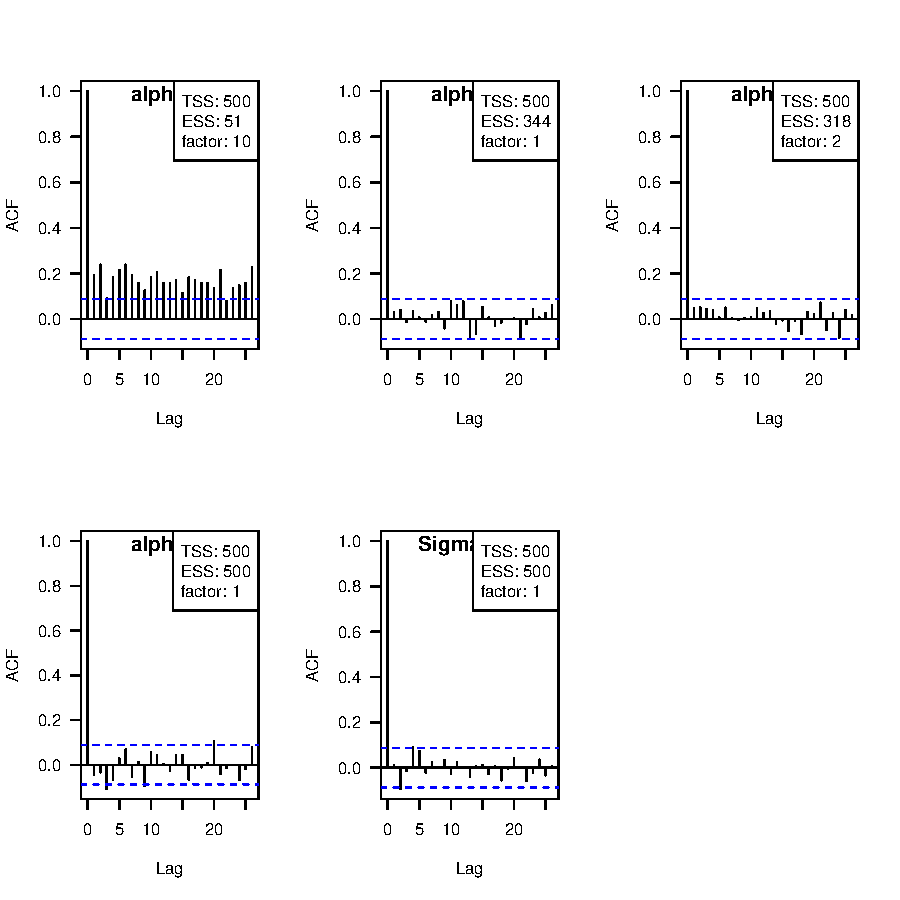
\includegraphics{rprobitb_oelschlaeger_bauer-plot-acf-model-train}

Here, the effective sample size is the value $\text{TSS} / (1 + \sum_{k\geq 1} \rho_k)$, where $\rho_k$ is the auto correlation between the chain offset by $k$ positions. The auto correlations are estimated via the \fct{stats::acf} function.

\subsection{Model transformation after estimation} \label{subsec:model_transformation}

The \fct{transform} method can be used to transform an \class{RprobitB\_fit} object in three ways:

1. change the length \code{B} of the burn-in period, for example
\begin{Schunk}
\begin{Sinput}
> model_train <- transform(model_train, B = 1)
\end{Sinput}
\end{Schunk}

2. change the thinning factor \code{Q} of the Gibbs samples, for example
\begin{Schunk}
\begin{Sinput}
> model_train <- transform(model_train, Q = 100)
\end{Sinput}
\end{Schunk}

3. or change the model normalization \code{scale}, for example
\begin{Schunk}
\begin{Sinput}
> model_train <- transform(model_train, scale = list(parameter = "s", index = 1, value = 1))
\end{Sinput}
\end{Schunk}

\section{Modeling heterogeneity} \label{sec:modeling_heterogeneity}

\section{Choice prediction} \label{sec:choice_prediction}

\section{Model selection} \label{sec:model_selection}


\section{Applications} \label{sec:applications}


\subsection{Chess opening choice} \label{subsec:chess_opening_choice}

\subsection{Berserking choice in online chess} \label{subsec:berserk}

\subsection{Child wish} \label{subsec:child_wish}

\subsection{Contraception choice} \label{subsec:contraception_choice}


\section{Conclusion} \label{sec:conclusion}

%% The problem
This paper addressed the problem of specifying mixing distributions in the multinomial probit model with a panel data setting, constituting an important part of the model selection for which the literature does not provide much guidance so far. In the absence of alternatives, many applications of the mixed multinomial probit model rely on different types of standard parametric distributions for modelling heterogeneity in preferences in combination with a likelihood-value based model selection. This course of action is very restrictive and imposes strong assumptions on the distribution of the model parameters that could potentially lead to misspecification and biased estimates.

%% Our solution
We proposed a new approach that improves the current specification strategies in several ways: First, our approach does not require any distributional assumption, since the latent class setting is flexible enough to approximate practically any distribution shape and allowing for any correlation pattern. Second, the weight-based updating scheme ensures that the number of latent classes does not need to be prespecified. Third, the imposed Bayesian estimation framework avoids many numerical problems that occur in the frequentist approach. Most notably, no likelihood function has to be evaluated nor approximated. Comparing the numerical estimation speed to the non-parametric frequentist approach of \cite{Bauer:2019}, we found that our implementation of the Bayesian approach is at least 10 times faster. The improvement becomes more distinct for panel data settings with a high number of choice occasions. This is due to the fact that for given total sample size $NT$ a large $T$ is beneficial for the Bayesian approach as then the number of vectors $\beta_n,~ n = 1,...,N$ is comparatively small, while in the frequentist approach calculating the likelihood becomes more challenging for increasing the number $T$ of choice situations faced by each of the $N$ individuals. On the other hand, the grid based frequentist approach of \cite{Bauer:2019} can potentially achieve a better approximation (especially of point masses) due to the relatively high number of latent classes. However, this approach requires that a suitable grid is set prior to the estimation with a specification of upper bounds for the coefficients. Additionally, the curse of dimensionality plays a crucial role, which is less of a burden in the Bayesian approach. Note that for a fully specified parametric structure these concerns do not play such a big role also for the frequentist approach.

%% Planned extensions
Our simulation results verified that the proposed approach achieves good approximations of the mixing distribution in common choice modelling situations, where the underlying heterogeneity cannot be captured by standard parametric distributions. It would be interesting to apply the approach also to empirical data in the future. Additionally,
further research on how to properly address sign-restricted coefficients is required.


\section*{Computational details}

The results in this paper were obtained using
\proglang{R}~4.1.3 with the
\pkg{RprobitB}~1.0.0.9000 package. \proglang{R} itself
and all packages used are available from the Comprehensive
\proglang{R} Archive Network (CRAN) at \url{https://CRAN.R-project.org/}.


\section*{Acknowledgments}

This work has been financed partly by the Deutsche Forschungsgemeinschaft (DFG, German Research Foundation) - Projektnummer 356500581 which is gratefully acknowledged.

\bibliography{ref}


\end{document}
